\chapter{Synthesis}
\label{chap:synthesis}

This chapter describes the problem statement, its definition, and the approaches
that were studied in order to solve it. The first one, described in
section~\ref{sec:first-approach}, is based on a component-based constraint
solving approach first applied to the synthesis of bitvector
programs~\cite{Gulwani:2011:SLP, Jha:oracle:2010}.

\section{Problem Description}
\label{sec:problem-description}

We are working in the context of the OutSystems platform. OutSystems is a
low-code platform that features visual application development, easy integration
with existing systems, and the possibility to add own code when needed. To that
effect, the kind of programs we are interested in are expressions in the
OutSystems language
\footnote{\url{https://success.outsystems.com/Documentation/11/Reference/OutSystems_Language/Logic/Expressions}}.

We can think of OutSystems expressions as a simple functional language of
operands and operators that compose themselves to create pure, stateless,
loop-less programs. This means that OutSystems expressions do not have
side-effects, like printing to the screen, or writing to a database, and do not
permit any variables or (for/while) loops. They do, however, have conditional
expressions in the form of ``if'' statements. The library of builtin expressions
includes functions that manipulate builtin data types such a text strings,
numbers, or dates
\footnote{\url{https://success.outsystems.com/Documentation/10/Reference/OutSystems_Language/Data/Data_Types/Available_Data_Types}}
\footnote{\url{https://success.outsystems.com/Documentation/10/Reference/OutSystems_Language/Logic/Built-in_Functions}}.

\begin{table}[]
  \noindent\makebox[\textwidth]{
    \begin{tabular}{@{}ll@{}}
      \toprule

      \multicolumn{1}{c}{Function Signatures}
      & \multicolumn{1}{c}{Description}
      \\ \midrule

      Concat(t: Text, s: Text): Text
      & Concatenation of the texts \textit{t} and \textit{s}.
      \\ \midrule

      Index(t: Text, s: Text, n: Integer): Text
      & \begin{tabular}{@{}l@{}}
          Retrieves first position of \textit{s} at or after \textit{n}
          characters in t.\\
          Returns -1 if there are no occurrences of \textit{s} in \textit{t}.
        \end{tabular}
      \\ \midrule

      Length(t: Text): Integer
      & Returns the number of characters in \textit{t}.
      \\ \midrule

      Replace(t: Text, s: Text, s': Text): Text
      & Returns \textit{t} after replacing all occurrences of \textit{s} with
        \textit{s'}.
      \\ \midrule

      Substr(t: Text, i: Integer, n: Integer): Text
      & Returns the substring of \textit{t} with \textit{n} characters starting
        at index \textit{i}.
      \\ \midrule

      ToLower(t: Text): Text
      & Converts all characters in \textit{t} to lowercase.
      \\ \midrule

      ToUpper(t: Text): Text
      & Converts all characters in \textit{t} to uppercase.
      \\ \midrule

      Trim(t: Text): Text
      & Removes all leading and trailing space characters (' ') from \textit{t}.
      \\ \midrule

      TrimStart(t: Text): Text
      & Removes all leading space characters (' ') from \textit{t}.
      \\ \midrule

      TrimEnd(t: Text): Text
      & Removes all trailing space characters (' ') from \textit{t}.
      \\ \midrule

      +(x: Integer, y: Integer): Integer
      & Integer addition.
      \\ \midrule

      -(x: Integer, y: Integer): Integer
      & Integer subtraction.
      \\ \bottomrule
    \end{tabular}}
  \caption{Description of the builtin functions used for synthesis.}
  \label{table:builtin-description}
\end{table}

\begin{table}[]
  \noindent\makebox[\textwidth]{
    \begin{tabular}{@{}ll@{}}
      \toprule

      \multicolumn{1}{c}{Function Signatures}
      & \multicolumn{1}{c}{Examples}
      \\ \midrule

      Concat(t: Text, s: Text): Text
      & \begin{tabular}[c]{@{}l@{}}
          Concat("", "") = ""\\
          Concat("x", "yz") = "xyz"
        \end{tabular}
      \\ \midrule

      Index(t: Text, s: Text, n: Integer): Text
      & \begin{tabular}[c]{@{}l@{}}
          Index("abcbc", "b", 0) = 1\\
          Index("abcbc", "b", 2) = 3\\
          Index("abcbc", "d", 0) = -1
        \end{tabular}
      \\ \midrule

      Length(t: Text): Integer
      & \begin{tabular}[c]{@{}l@{}}
          Length("") = 0\\
          Length("abc") = 3
        \end{tabular}
      \\ \midrule

      Replace(t: Text, s: Text, s': Text): Text
      & Replace("ababa", "a", "xy") = "xybxybxy"
      \\ \midrule

      Substr(t: Text, i: Integer, n: Integer): Text
      & \begin{tabular}[c]{@{}l@{}}
          Substr("abcdef", 2, 3) = "cde"\\
          Substr("abcdef", 2, 100) = "cdef"
        \end{tabular}
      \\ \midrule

      ToLower(Text): Text
      & ToLower("AbC ") = "abc "
      \\ \midrule

      ToUpper(Text): Text
      & ToUpper("aBc ") = "ABC "
      \\ \midrule

      Trim(Text): Text
      & Trim("    xyz    ") = "xyz"
      \\ \midrule

      TrimStart(Text): Text
      & TrimStart("    xyz    ") = "xyz    "
      \\ \midrule

      TrimEnd(Text): Text
      & TrimEnd("    xyz    ") = "    xyz"
      \\ \midrule

      % Add(x: Integer, y: Integer): Integer
      % & \begin{tabular}[c]{@{}l@{}}
      %     Add(0, 0) = 0
      %     Add(1, 2) = 3
      %   \end{tabular}
      % \\ \midrule

      % Sub(x: Integer, y: Integer): Integer
      % & \begin{tabular}[c]{@{}l@{}}
      %     0 - 0 = 0
      %     1 - 2 = -1
      %   \end{tabular}
      % \\ \bottomrule
    \end{tabular}}
  \caption{Examples for the builtin functions used for synthesis.}
  \label{table:builtin-examples}
\end{table}

In this work we are mainly interested in synthesizing expressions that
manipulate text strings, like concatenation, substring slicing or whitespace
trimming. As some of these operations involve indexing, we are also interested
in synthesizing simple arithmetic expressions involving addition and
subtraction. Therefore, the data types we are working with are text strings and
integers. In particular, we are not dealing neither with boolean or conditional
expressions. Table~\ref{table:builtin-description} describes the builtin
expressions that our synthesized programs can be composed of.
Table~\ref{table:builtin-examples} shows input-output examples for each of the
functions in Table~\ref{table:builtin-description}.

\begin{example}
  Suppose that we would like to capitalize a given text string \textit{t}. For
example, given the text ``joseph'' we would like to obtain ``Joseph''. The
expression

% \texttt{f(x) = ToUpper(Substr(x, 0, 1)) + Substr(x, 1, Length(x))}

\begin{center}
\begin{tabular}{l}
\texttt{f(x) = ToUpper(Substr(x, 0, 1)) + Substr(x, 1, Length(x))}\\
\end{tabular}
\end{center}

\noindent
satisfies this example.
\end{example}


% TODO Example of one or more outsystems expressions.
% Include one or more where there are constants that are not part of the inputs,
% and explain that it would be nice if the synthesizer could do that for us.
\todo{Listing x includes examples of outsystems expressions. These do y and z.}{}





\section{A First Approach}
\label{sec:first-approach}

In our context, we are working in a \gls{pbe} setting, so we are interested in
synthesizing an OutSystems expression from a set of input-output examples
$\{(I_i, o_i)\}_i$.

Because OutSystems expressions are composed of self-contained pure functions,
this synthesis problem fits nicely in the component-based synthesis paradigm.
Therefore assume we are given a \textit{library} of base components $F$ that the
synthesizer can use in order to make the programs. These components will be the
builtin functions drawn from the OutSystems library. Each component can take a
finite number of inputs and return exactly one output. The allowed types for the
inputs and the output are \todo{text strings and integers}{expand?}.

More formally, a component $f \in F$ is represented by an expression
$\phi{}_f$ that specifies how its input parameters $P_f$ relate to its
return value $r_f$.

% TODO Add an example of one or two components and their possible specs

% FIXME fix the literals
OutSystems expressions can also have constant literals, like
\lstinline{"string"}, or \lstinline{0}. These can either be given by the user as
extra information, or figured out automatically by the synthesizer.

If we ignore well-typedness, an OutSystems expression is a tree-like program
whose form can be succintly described using a \gls{cfg}:

\begin{center}
  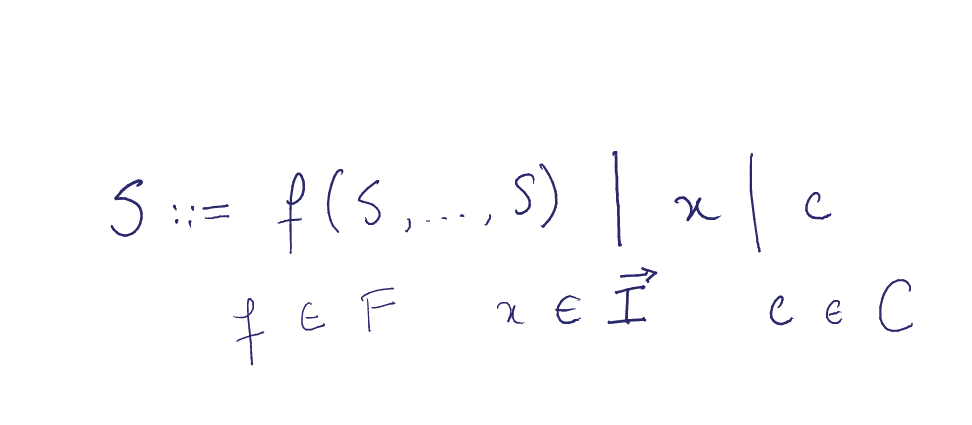
\includegraphics[width=0.7\textwidth]{assets/cfg-expressions.png}
\end{center}

% TODO Show grammar here.

where $I$ denotes the set of inputs from a given input-output example, and
$C$ is the set of constant literals in the OutSystems language.

It is useful to reason about OutSystems expressions in another representation,
called \gls{ssa}. A program in \gls{ssa} form is a line program with variables
where every variable is assigned exactly once and defined before its use. For
example, the program from Figure ??? could be written in \gls{ssa} form in the
following manner:

% TODO Show program in SSA form

This program format can be described succintly with the following \gls{cfg}:

% TODO Show cfg for programs in SSA form
$S ::= y \leftarrow c | y \leftarrow f(x_1, ..., x_n) | S;S$

The non-terminal $S$ represents a line in the program. A line is an assignment
of a variable to a constant literal $c$ or to the return value of a component
$f$ on inputs $x_1, ..., x_n$. Thus, the structure of a program in \gls{ssa}
form is a sequence of assignments.

The approach described in this section is based on
\citeauthor{Jha:oracle:2010}'s program encoding. The idea is to encode the
program space in a formula that is then constrained further in order to encode
only those programs that satisfy the input-output examples. A solution to this
formula can then be decoded back yielding a program that satisfies the set of
examples.

The synthesizer follows the \gls{ogis} model, described in
Section~\ref{sec:ogis}. It has a learner part and an oracle part, which will
call here the \textit{enumerator} and the \textit{solver}, respectively.

The enumerator receives the input-output examples as input, and is parameterized
by the library of base components. The enumerator is responsible for drawing a
subset of components from the library. It then passes these components to the
solver, along with the input-output examples, and queries whether there is any
program made only of those components that satisfies the examples. There is an
additional restriction that the program must use each of the components exactly
once.

% TODO Explain how the enumerator draws the components

The solver works by encoding the query into an \gls{smt} formula, and uses an
automated SMT solver to check for satisfiability. The SMT solver might or might
not be able to solve the formula. If the formula is satisfiable, the solver
responds to the enumerator with SAT and a solution to that formula. If not, it
responds UNSAT or UNKNOWN, depending on whether the formula is unsatisfiable or
the SMT solver could not verify its satisfiability, respectively.

The procedure finishes when enumerator receives SAT from the solver: the
enumerator decodes the solution to the formula into an actual program, and
outputs it.

% TODO Insert here a listing of the program

\subsection{Encoding}
\label{sec:encoding}

\todo{TODO}{}

``Each connection is encoded using an integer-valued location variable.''

\(N = |I| + |C|\)

Formula for syntactically well-formed programs:

\begin{align*}
  \phi{}_{wfp} &= \bigwedge_{f \in F}\bigwedge_{p \in P_f} (1 \leq l_p \leq l_f) \\
  &\wedge \bigwedge_{f \in F} (N + 1 \leq l_f \leq N + |F|) \\
  &\wedge \bigwedge_{\substack{r_1, r_2 \in R\\ r_1 \not\equiv r_2}} (l_{r_1} \neq l_{r_2})
   \wedge \bigwedge_{\substack{r_1, r_2 \in R\\ r_1 \not\equiv r_2}} (l_{r_1} \neq l_{r_2}) \\
  &\wedge \bigwedge_{p \in P}\bigwedge_{\substack{x \in I \cup C \cup R \cup \{o\} \\ kind(p) \neq kind(x)}} (l_p \neq l_x)
   \wedge \bigwedge_{\substack{r \in R \\ kind(r) \neq kind(o)}} (l_r \neq l_o)
\end{align*}

Semantics:

\begin{align*}
  \phi{}_{spec} &= \bigwedge_{f \in F} \phi{}_f (I_f, o_f) \\
  \phi{}_{flow} &= \bigwedge_{p \in P}\bigwedge_{\substack{x \in I \cup C \cup R \\ kind(p) \neq kind(x)}} (l_p = l_x \implies p = x)
\end{align*}

All inputs used:

\[ \phi{}_{in} = \bigwedge_{i \in I}\bigvee_{p \in P}(l_i = l_p) \]

All outputs used:

\begin{align*}
  \phi{}_{out} &= \bigwedge_{f \in F}\bigvee_{p \in P - P_f}(l_f = l_p) \\
               &\vee \bigwedge_{f \in F} (l_f = l_o)
\end{align*}

Constrain the length of string constants:

\[
  \phi{}_{len} = \bigwedge_{\substack{c \in C \\ kind(c) = string}} len(c) \leq 5
\]

Extra:

\[ \phi{}_{extra} = \phi{}_{in} \wedge \phi{}_{out} \wedge \phi{}_{len} \]

Formula for a single run of a program:

\begin{align*}
  \phi{}_{prog} = \exists P,R\ldotp (\phi{}_{wfp} \wedge \phi{}_{spec} \wedge
  \phi{}_{flow} \wedge \phi{}_{extra})
\end{align*}

The full formula:

\[
  \Phi{} = \exists L\ldotp \bigwedge_{(I, o) \in E}\phi{}_{prog}
\]

We could also try:

\[
  \Phi{} = \exists L\ldotp \forall (I, o) \in E \ldotp \phi{}_{prog}
\]

\[
  \Phi{} = \exists L\ldotp \forall I, o \ldotp (I, o) \in E \implies \phi{}_{prog}
\]



% TODO Concrete example of the encoding of a program